\section{The exact solution for MQ NMR dynamics for a three-spin system in a nanopore at low temperatures}
\label{sec:exact_sol}

We consider a system of $N=3$ spins coupled through the Hamiltonian $H_{MQ}$ of Eq.   (\ref{eq:ham_mq}). The possible values $S$ of the total spin angular momentum are $\frac 3 2$ and $\frac 1 2$. One can find that the matrix representation of $H_{MQ}^{3/2}$  is 

\begin{equation}
    \label{eq:ham_3_2}
    H_{MQ}^{3/2} = 
    \begin{pmatrix}
        0 & 0 & -\frac{\sqrt{3} D}{2} & 0 \\
        0 & 0 & 0 & -\frac{\sqrt{3} D}{2} \\
        -\frac{\sqrt{3} D}{2} & 0 & 0 & 0 \\
        0 & -\frac{\sqrt{3} D}{2} & 0 & 0 
    \end{pmatrix}.
\end{equation}
The eigenvalues $\lambda_{3/2}^{(i)}(i=1, 2, 3, 4)$ of  $H_{MQ}^{3/2}$ are the following 
\begin{align}
    \label{eq:eigvals_3_2}
    \lambda_{3/2}^{(1)} &= -\frac{\sqrt{3} D}{2}, \quad
    \lambda_{3/2}^{(2)} = -\frac{\sqrt{3} D}{2}, \notag \\
    \lambda_{3/2}^{(3)} &= \frac{\sqrt{3} D}{2}, \quad
    \lambda_{3/2}^{(4)} = \frac{\sqrt{3} D}{2}.
\end{align}
The appropriate set of eigenvectors reads as follows:

\begin{align}
    \label{eq:eigvecs_3_2}
    u_{3/2}^{(1)} & =  \left(\frac{1}{\sqrt{2}}, 0, 
                   \frac{1}{\sqrt{2}}, 0\right) ,
    \notag \\
    u_{3/2}^{(2)} & =  \left(0, \frac{1}{\sqrt{2}}, 
                   0, \frac{1}{\sqrt{2}}\right) ,
    \notag \\
    u_{3/2}^{(3)} & =  \left(-\frac{1}{\sqrt{2}}, 0, 
                   \frac{1}{\sqrt{2}}, 0\right) ,
    \notag \\               
    u_{3/2}^{(4)} & =  \left(0, -\frac{1}{\sqrt{2}}, 
                   0, \frac{1}{\sqrt{2}}\right)  .              
\end{align}
The block $H^{1/2}_{MQ}$ is a scalar
\begin{equation}
    \label{eq:ham_1_2}
    H^{1/2}_{MQ} = 0.
\end{equation}
The solution of Eq.   (\ref{eq:liouvile}), $\rho_{\alpha}^{n/2} (\tau) \quad (n = 1, 3; \, \alpha = \mathrm{LT}, \mathrm{HT})$, where the Hamiltonian $H_{MQ}$ is replaced by the Hamiltonian $H_{MQ}^{n/2}$, is 

\begin{equation}
    \label{eq:liouvile_sol}
    \rho_{\alpha}^{n/2}(\tau) = 
    U_{n/2} e^{-i\Lambda^{n/2}\tau} U^{+}_{n/2}
    \rho^{n/2}_{\alpha}(0)
    U_{n/2} e^{i\Lambda^{n/2}\tau} U^{+}_{n/2},
\end{equation}
where $\Lambda^{n/2}$ is the diagonal matrix of the eigenvalues and $U_{n/2}$ is the matrix of the eigenvectors of the block $H_{MQ}^{n/2} \quad (n=1, 3)$, and the initial density matrices $\rho_\mathrm{LT}^{n/2}(0)(\alpha=LT)$ and $\rho_\mathrm{HT}^{n/2}(0)(\alpha=HT)$ are the following:

\begin{align}
    \label{eq:rho_LT_init}
    \rho_\mathrm{LT}^{3/2}(0) &= \dfrac 1 Z
    \begin{pmatrix}
        e^{\frac{3b}{2}} & 0 & 0 & 0 
        \\
        0 & e^{\frac{b}{2}} & 0 & 0 
        \\
        0 & 0 & e^{-\frac{b}{2}} & 0 
        \\
        0 & 0 & 0 & e^{-\frac{3b}{2}}
    \end{pmatrix}, 
    \notag \\
    \rho_\mathrm{LT}^{1/2}(0) &= \dfrac 1 Z
    \begin{pmatrix}
        e^{\frac{b}{2}} & 0 
        \\
        0 & e^{-\frac{b}{2}}
    \end{pmatrix},
\end{align}

\begin{align}
    \label{eq:rho_HT_init}
    \rho_\mathrm{HT}^{3/2}(0) & = 
    \begin{pmatrix}
        \frac{3}{2} & 0 & 0 & 0 
        \\
        0 & \frac{1}{2} & 0 & 0 
        \\
        0 & 0 & -\frac{1}{2} & 0 
        \\
        0 & 0 & 0 & -\frac{3}{2}
    \end{pmatrix},
    \notag \\
    \rho_\mathrm{HT}^{1/2}(0) &= 
    \begin{pmatrix}
        \frac{1}{2} & 0 
        \\
        0 & -\frac{1}{2}
    \end{pmatrix}.
\end{align}
After a calculation using Eqs.  (\ref{eq:eigvals_3_2}), (\ref{eq:eigvecs_3_2}), (\ref{eq:liouvile_sol}), (\ref{eq:rho_LT_init}), and (\ref{eq:rho_HT_init}) with $n = 3$, one obtains 
\begin{equation}
    \label{eq:rho_HT_eval_3_2}
    \rho_\mathrm{HT}^{3/2}(\tau) =
    \begin{pmatrix}
            \xi + \frac 1 2  
        & 
            0 
        & 
            -i\eta 
        & 
            0 
        \\
            0 
        & 
            \xi - \frac 1 2 
        & 
            0 
        & 
            -i\eta
        \\
            i\eta 
        &
            0 
        & 
            -\xi + \frac 1 2  
        & 
            0 
        \\
            0 
        & 
            i\eta 
        & 
            0 
        & 
            -\xi - \frac 1 2 
    \end{pmatrix},
\end{equation}
where 
\begin{equation}
    \xi = \cos(\sqrt{3}D\tau), \quad 
    \eta = \sin(\sqrt{3}D\tau), 
\end{equation}
and
\begin{multline}
    \label{eq:rho_LT_eval_3_2}
    \rho_\mathrm{LT}^{3/2}(\tau) = \frac{1}{Z} \\
    \begin{pmatrix}
            ue^{-\frac{b}{2}} + ve^{\frac{3b}{2}}
        & 
            0 
        & 
            -ie^{\frac{b}{2}}w
        & 
            0 
        \\
            0 
        & 
            ue^{-\frac{3b}{2}} + ve^{\frac{b}{2}} 
        & 
            0 
        & 
            -ie^{-\frac{b}{2}}w 
        \\
            ie^{\frac{b}{2}}w
        &
            0 
        & 
            ue^{\frac{3b}{2}} + ve^{-\frac{b}{2}}
        & 
            0 
        \\
            0 
        & 
            ie^{-\frac{b}{2}}w
        & 
            0 
        & 
            ue^{\frac{b}{2}} + ve^{-\frac{3b}{2}}
    \end{pmatrix},
\end{multline}
where
\begin{align}
    u & =  \sin^2\left(\frac{\sqrt{3}}{2}D\tau\right), \notag \\
    v & =  \cos^2\left(\frac{\sqrt{3}}{2}D\tau\right), \notag \\
    w & =  \sin(b)\sin\left(\sqrt{3}D\tau\right). 
\end{align}

An analogous calculation for the matrices $\rho^{1/2}_\mathrm{HT} (\tau)$ and $\rho^{1/2}_\mathrm{LT} (\tau)$ using Eqs.   (\ref{eq:liouvile_sol}), (\ref{eq:rho_LT_init}), and (\ref{eq:rho_HT_init}) yields

\begin{equation}
    \label{eq:rho_HT_eval_1_2}
    \rho_\mathrm{HT}^{1/2}(\tau) = 
    \begin{pmatrix}
            \frac 1 2  
        & 
            0  
        \\
            0
        & 
            -\frac 1 2   
    \end{pmatrix},
\end{equation}

\begin{equation}
\label{eq:rho_LT_eval_1_2}
    \rho_\mathrm{LT}^{1/2}(\tau) = \frac 1 Z 
    \begin{pmatrix}
            e^{\frac b 2}
        & 
            0  
        \\
            0
        & 
            e^{-\frac b 2}  
    \end{pmatrix}.
\end{equation}

Only the MQ NMR coherences of the zeroth and plus/minus second orders appear in the considered systems. These intensities can be calculated with Eqs.   (\ref{eq:coherence_k_s}) and (\ref{eq:rho_HT_eval_3_2}) - (\ref{eq:rho_LT_eval_1_2}):
\begin{align}
    \label{eq:analit_res_coherence}
    J_0(\tau) & = \dfrac{2\cos^2(\sqrt{3}D\tau) + 1}{3}, \notag \\
    J_{\pm 2}(\tau) & = \dfrac{\sin^2(\sqrt{3}D\tau)}{3} .
\end{align}

One can check that the sum of the intensities of Eq.   (\ref{eq:analit_res_coherence}) equals 1 independently of $\tau$ in accordance with Eq.   (\ref{eq:sum_of_coherence}). The profiles of the calculated intensities $J_n(\tau)$, n=0,2 are shown in Fig.\ref{fig:exact_j}.
\begin{figure}
    \centering
    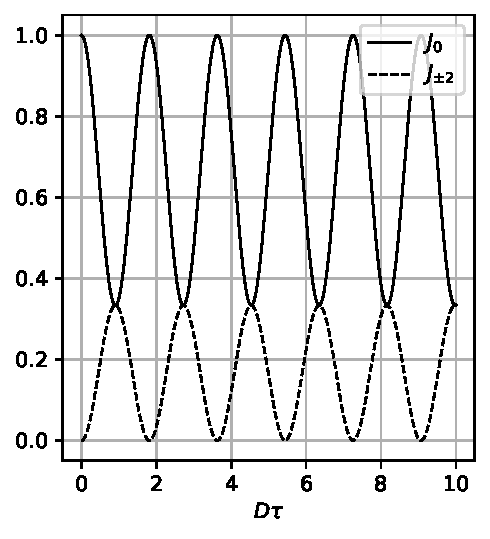
\includegraphics{src/exact_j.pdf}
    \caption{Intensities of MQ NMR coherences $J_n, \quad n=0, 2$ in a nanopore with $N = 3$.}
    \label{fig:exact_j}
\end{figure}
